\documentclass[a4paper,11pt]{article}
%\usepackage[utf8]{inputenc}

\usepackage{pdfpages}
\usepackage{mathtools}
\usepackage{amsmath}
\usepackage{amssymb}
\usepackage{tikz}
\usepackage{physics}

\newcommand{\Mypm}{\mathbin{\tikz [x=1.4ex,y=1.4ex,line width=.1ex] \draw (0.0,0) -- (1.0,0) (0.5,0.08) -- (0.5,0.92) (0.0,0.5) -- (1.0,0.5);}}%




\newcommand\underrel[3][]{\mathrel{\mathop{#3}\limits_{%
      \ifx c#1\relax\mathclap{#2}\else#2\fi}}}

\numberwithin{equation}{section}
\numberwithin{figure}{section}
\usepackage{graphicx}
\setlength{\parindent}{0cm}

\title{Quantum fields in de Sitter space}
\author{Ben Sanby}

\usepackage{geometry}
\geometry{a4paper, left=25mm, right=25mm, top=30mm, bottom=25mm}

\renewcommand{\baselinestretch}{1.2}

\begin{document}
\begin{large}

\clearpage
\maketitle
\thispagestyle{empty}
\begin{figure}[h]
    \centering
    \vspace{100mm}
    
\includegraphics[width=0.2\columnwidth]{kcl_logo.png}
\end{figure}

\newpage

\begin{abstract}
    This paper starts by reviewing the geometry of the de Sitter spacetime focusing on the isometries generated by Killing vectors. We also look at different metrics that are restricted to specific regions of the spacetime, and find that in the late time limit the symmetries give a similar local structure to that of ${\rm I\!R}^3$. We then look at solving the classical Klein Gordon equation in this spacetime and find that the energy is not a conserved quantity. The solutions to the Klein Gordon equation give some interesting results which could allow for observations from the early inflationary era. Finally we reach the main aim of the paper, which is to review a quantized scalar field in the de Sitter background, we work through the solutions to the two point function and review their behaviour in the early and late time limits.
\end{abstract}

\newpage

\tableofcontents


\newpage

\section{Introduction}

We begin by considering the motivation of why we would like to look at quantum fields in de Sitter space, after all, exploring abstract mathematical ideas can give an unforeseen insight into areas of physics that we may not have previously considered, however there are plenty of unexplored areas of maths and physics that have physical reward in researching so as to better understand the universe we live in. Experimental data shows our universe is expanding, not only that but at an accelerating rate \cite{supernova1,supernova2}. We find our universe has a small, but non zero, positive cosmological constant \cite{cosmoconst} driving this expansion, which if it remains positive will see the dilution of the large scale structure we see today and the rise of the popularly referred to ``big chill" or ``big freeze" \cite{future structure}. We also see this expansion of our universe in the inflationary era \cite{inflation1,inflation2} not long after the Big Bang, some of these models source an inflationary scalar field, which can be affected by quantum fluctuations. So with these two periods of expansion where our universe appears approximately de Sitter, the motivation for the study of this geometry and the effects of quantum interactions in such a space become quite obvious. The aim of this paper is therefore, to build a foundation of what it means for a spacetime to be de Sitter, and then present a quantum field theory in this background and compare the solutions to that of flat space.


\newpage 


\section{de Sitter spacetime}


We will start by looking at the geometry of the sphere, then identify the similarities shared with the de Sitter geometry to gain a better understanding of the background spacetime that we are working in. 

\vspace{0.5cm}

\subsection{$dS_2$}


Initially we will look at the geometry in $dS_2$ as it is easier to understand the concepts in lower dimensions, and then it becomes quite intuitive to generalise to higher dimensions; the spacetime we are working toward understanding is $dS_4$.


\subsubsection{Killing vectors}


Killing vectors are generated by isometries and can be found by solving the Killing equation

$$(\mathcal{L}_Xg)_{ij} \coloneqq X^k \partial _k g_{ij} + \partial _i X^l g_{lj} + \partial _j X^l g_{li}  = 0 $$


where $\mathcal{L}$ is the Lie derivative, $X$ is the Killing vector field and $g$ is the metric. However it can get quite complicated to solve the Killing equation for certain metrics, which is why we can make it easier to find the Killing vectors by transforming coordinates from a system where we already know the Killing vectors to our desired system, rather than repeatedly solving the Killing equation. To demonstrate this we can look at the simple example of the standard metric and the round metric on ${\rm I\!R}^3$.

The standard metric on ${\rm I\!R}^3$ is $ds^2=dx^2+dy^2+dz^2$, so $g_{ij}=\delta_{ij}$, it is not difficult to find the Killing vectors which can be presented in the basis

\begin{equation}
\label{eq:translation}
    \partial_i
\end{equation}

\begin{equation}
\label{eq:rotation}
    \epsilon_{ijk}x^i\partial^j
\end{equation}


where $i=1,2,3$ and repeated indices are summed. We note that the commutators of these Killing vector fields closes on itself, and so it forms a Lie group which is that of the special Euclidean group. The first 3 Killing vectors Eq. \eqref{eq:translation} represent translations, and the second 3 Eq. \eqref{eq:rotation} represent rotations. As mentioned earlier, isometries generate Killing vectors. The definition of an isometry is a coordinate transformation that leaves the metric unchanged, because it is obvious that the distance between 2 points in ${\rm I\!R}^3$ does not change under translations or rotations, they are intuitively Killing vectors.

The maximal number of Killing vectors in d-dimensions is $\frac{d(d+1)}{2}$, meaning for ${\rm I\!R}^3$ there are 6, and as we have found 6, ${\rm I\!R}^3$ is therefore maximally symmetric.


\newpage


\subsubsection{Classical geometry of the sphere}


We will now take a look at the geometry of the sphere. The equation for the unit sphere is given by $x^2+y^2+z^2=1$, our aim is to embed the coordinates onto the sphere, we proceed by changing to polar coordinates

\begin{equation}
\label{eq:xpol}
    x=R\cos\theta\cos\phi 
\end{equation}

\begin{equation}
\label{eq:ypol}
    y=R\cos\theta\sin\phi 
\end{equation}

\begin{equation}
\label{eq:zpol}
    z=R\sin\theta
\end{equation}


where $R=1$ as we are looking at the unit sphere. We can then calculate the new metric by solving $dx^i=\frac{\partial x^i}{\partial \theta}d\theta+\frac{\partial x^i}{\partial \phi}d\phi$, where $x^i=\{x,y,z\}$, then substituting into the standard metric on ${\rm I\!R}^3$, giving $ds^2=d\theta^2+\cos^2\theta d\phi^2$ commonly know as the round metric on the 2-sphere. 


\subsubsection{Isometries of the sphere}


We notice that by embedding the coordinates onto the 2-sphere we have reduced the dimensions by 1 as the 2-sphere is a 2 dimensional manifold, which means that we no longer have 6 Killing vectors but $3$ $(=\frac{2(2+1)}{2})$.We find that by fixing the coordinates to the unit sphere the translations are no longer isometries, however the rotations remain isometries of the 2-sphere and they form the special orthogonal group $SO(3)$ (note here, that the real isometry group of the sphere is $O(3)$ not $SO(3)$. However $O(3)$ does not preserve chirality and there is not a loss of generality in requiring that the determinant is $+1$, meaning we identify the group of isometries for the sphere as $SO(3)$, this assumption will be used throughout the rest of the paper for all isometry groups as we are not interested in the discrete symmetries). As previously mentioned, to calculate the Killing vectors of the 2-sphere we use the coordinate transformation from the standard metric as solving the Killing equation for the round metric becomes tedious. 

First we calculate the partial derivatives

\begin{equation}
\label{eq:part}
    \frac{\partial}{\partial x^i}=\frac{\partial \theta}{\partial x^i}\frac{\partial}{\partial \theta}+\frac{\partial \phi}{\partial x^i}\frac{\partial}{\partial \phi}
\end{equation}

Which gives

\begin{equation}
\label{eq:xpart}
\frac{\partial}{\partial x}=-\sin\theta\cos\phi\frac{\partial}{\partial \theta}-\frac{\sin\phi}{\cos\theta}\frac{\partial}{\partial \phi}
\end{equation}


\begin{equation}
\label{eq:ypart}
\frac{\partial}{\partial y}=-\sin\theta\sin\phi\frac{\partial}{\partial \theta}+\frac{\cos\phi}{\cos\theta}\frac{\partial}{\partial \phi}
\end{equation}


\begin{equation}
\label{eq:zpart}
\frac{\partial}{\partial z}=\cos\theta\frac{\partial}{\partial \theta}
\end{equation}


\newpage


We then substitute into Eq. \eqref{eq:rotation} the values for: $x^i$ given by Eqs. \eqref{eq:xpol} to \eqref{eq:zpol}, and $\partial^j$ given by Eqs. \eqref{eq:xpart} to \eqref{eq:zpart}, to give

\begin{equation}
\label{eq:xyrot}
x\partial_y-y\partial_x=\partial_\phi
\end{equation}


\begin{equation}
\label{eq:yzrot}
y\partial_z-z\partial_y=\sin\phi \partial_\theta-\tan\theta\cos\phi \partial_\phi
\end{equation}


\begin{equation}
\label{eq:zxrot}
z\partial_x-x\partial_z=-\cos\phi \partial_\theta-\tan\theta\sin\phi \partial_\phi
\end{equation}


It is easy to show that these Killing vectors close under the Lie bracket.

\subsubsection{de Sitter geometry $dS_2$}


As we have reviewed the simple example of spherical geometry, we now proceed in a similar way for the de Sitter geometry. Instead of taking the standard metric on ${\rm I\!R}^3$ though we look at the Minkowski metric $ds^2=-dt^2+dx^2+dy^2$. It is obvious to see the similarity in the metrics as a simple coordinate transformation $t\xrightarrow[]{}iz$ gives the standard metric. To discuss the reason for embedding the coordinates of the standard metric onto the 2-sphere, the de Sitter geometry can be viewed as the embedding of the Minkowski metric onto the hyperboloid. 

\vspace{1.5cm}

\begin{figure}[h]
    \centering
    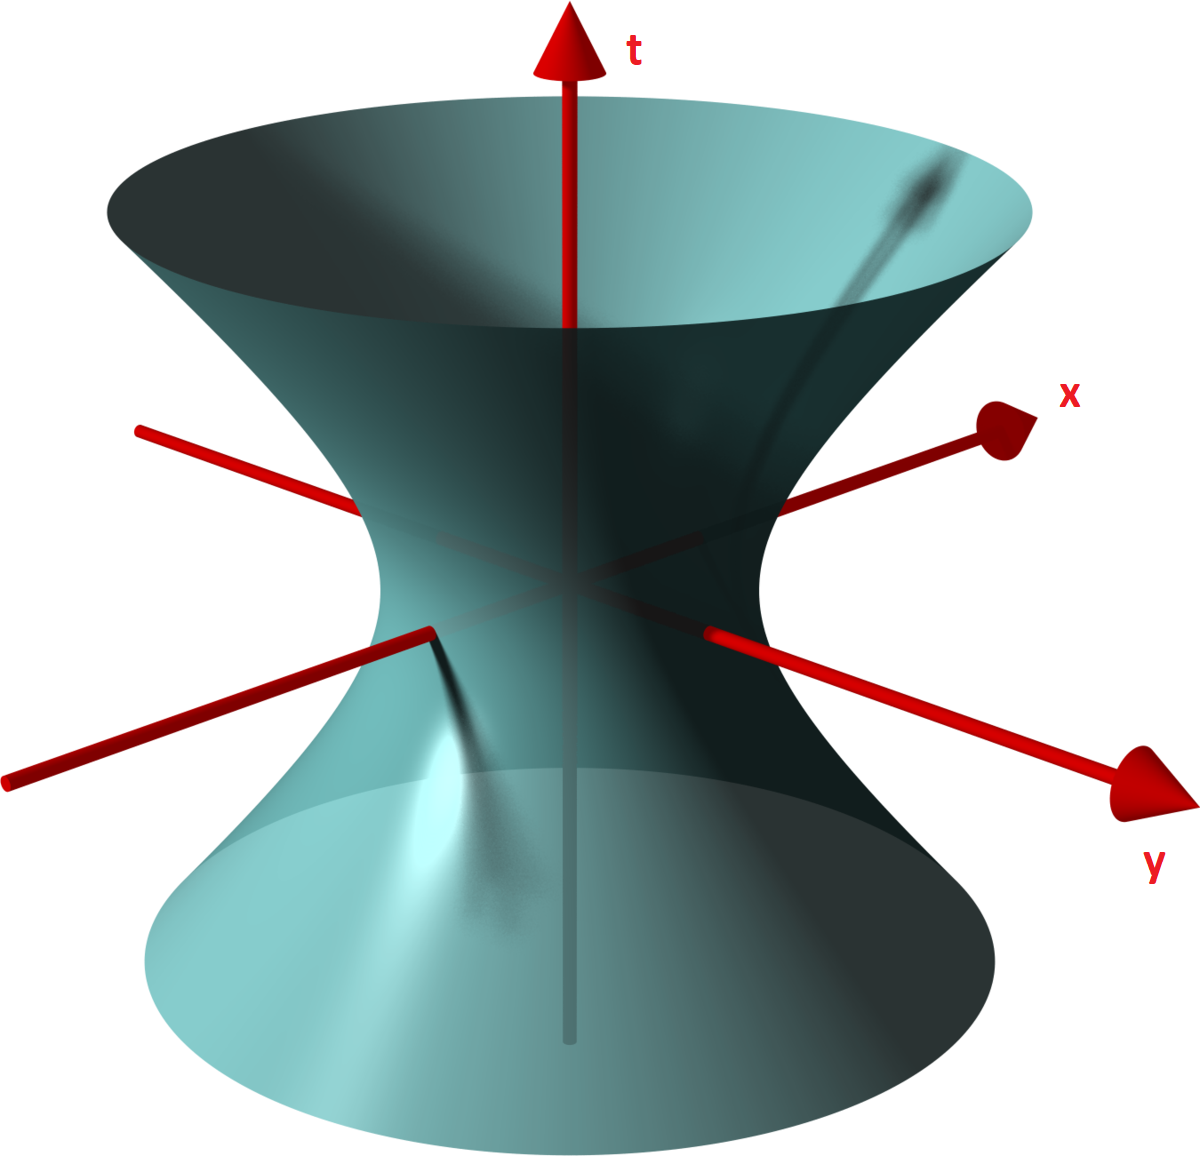
\includegraphics[width=8cm]{Hyperboloid.png}
    \caption{Hyperboloid surface}
    \label{fig:hyperboloid}
    
\end{figure}

\newpage

Proceeding in a similar fashion to the 2-sphere we can start by identifying the Killing vectors of Minkowski spacetime ${\rm I\!R}^{1,2}$. We realise the group structure we are looking for is the Poincar\'{e} group giving the Killing vectors

\begin{equation}
\label{eq:translation_dS}
    \partial_t
    \hspace{2cm}
    \partial_x
    \hspace{2cm}
    \partial_y
\end{equation}

\begin{equation}
\label{eq:boost}
    x\partial_t+t\partial_x 
    \hspace{3cm}
    y\partial_t+t\partial_y
\end{equation}

\begin{equation}
\label{eq:rotation_dS}
    x\partial_y-y\partial_x 
\end{equation}

we have 1 time translation and 2 spatial translations \eqref{eq:translation_dS}, 2 boosts \eqref{eq:boost} and 1 rotation \eqref{eq:rotation_dS} to give the 6 Killing vectors we expect of this 3 dimensional spacetime. Following a similar procedure as before, taking the metric $ds^2=-dt^2+dx^2+dy^2$ and embedding it onto the hyperboloid $-t^2+x^2+y^2=1$, using the coordinate transformations

\begin{equation}
\label{eq:t_hyp}
    t=\sinh T 
\end{equation}

\begin{equation}
\label{eq:x_hyp}
    x=\cosh T\cos\phi
\end{equation}

\begin{equation}
\label{eq:y_hyp}
    y=\cosh T\sin\phi
\end{equation}

we can calculate the new induced metric to be $ds^2=-dT^2+\cosh^2T d\phi^2$ which is the de Sitter metric $dS_2$, otherwise referred to as the global metric on $dS_2$. We notice that the only difference between this and the 2-sphere example is the simple coordinate transformation $z \rightarrow it$ and $\theta \rightarrow iT$ which highlights the similarities between the two geometries.

\subsubsection{Isometries of $dS_2$}

Now that we have our Killing vectors on ${\rm I\!R}^{1,2}$ and our embedding coordinates on the hyperboloid, we can look at finding the Killing vectors in $dS_2$. When embedding the coordinates we again find that we lose the translation isometries leaving us with the rotation and two boosts, which represented in this coordinate system, are


\begin{equation}
\label{eq:xyrot_dS}
x\partial_y-y\partial_x=\partial_\phi
\end{equation}


\begin{equation}
\label{eq:xboost}
x\partial_t+t\partial_x=\cos\phi \partial_T-\sin\phi\tanh T \partial_\phi
\end{equation}


\begin{equation}
\label{eq:yboost}
y\partial_t+t\partial_y=\sin\phi \partial_T+\cos\phi\tanh T\partial_\phi
\end{equation}

\vspace{0.5cm}

we identify this group as the Lorentz group in 2 spatial dimensions $SO(1,2)$.


\newpage


\subsubsection{Penrose diagram}

We now take a look at the Penrose diagram, which is similar to the Minkowski spacetime diagram in that the vertical direction represents time, the horizontal direction represents a spatial dimension, and the null geodesics are lines at $45^{\circ}$. The diagram is designed to capture the causal structure of the spacetime, the difference to that of the Minkowski diagram is that, locally, the actual metric of the spacetime is conformally equivalent to the metric on the diagram itself. This means the entire spacetime is represented on the diagram, and so the coordinate system used has to be compact, which means we first need to compactify our coordinates.

We notice that for our metric $ds^2=-dT^2+\cosh^2T d\phi^2$ the spatial coordinates $\phi$ are already compact, ranging from $0$ to $2\pi$. So we need only compactify the temporal coordinate, as $T$ ranges from $-\infty$ to $+\infty$. We resolve this problem by changing coordinates so the metric is of the form

\begin{equation}
\label{Pen_metric_form}
    ds^2=a^2(\tau)(-d\tau^2+d\phi^2)
\end{equation}

We take our global metric and require

\begin{equation}
\label{Glob=Pen}
    -dT^2+\cosh ^2 T d\phi^2=a^2(\tau)(-d\tau^2+d\phi^2)
\end{equation}


Which gives us $a=\cosh T$ and $dT=a d\tau$ leading to

\begin{equation}
\label{Int1}
    \int \frac{dT}{\cosh T}= \int d\tau
\end{equation}

Which is solved to give

\begin{equation}
\label{T_tau_rel}
    \tanh \frac{T}{2}=\tan \frac{\tau}{2}
\end{equation}


If we then differentiate this to find $dT$ in terms of $d\tau$ and $\tau$ we get

\begin{equation}
\label{dT_dtau_rel}
    dT=\frac{1}{\cos\tau}d\tau
\end{equation}

Meaning the metric is now 

\begin{equation}
\label{compact_global_metric}
    ds^2=\frac{1}{\cos^2\tau}(-d\tau^2+d\phi^2)
\end{equation}

All our coordinates are now compact, as $\tanh x \in (-1,1)$ for $x \in {\rm I\!R}$, and $\tan^{-1} x \in (-\frac{\pi}{4},\frac{\pi}{4})$ for $x \in (-1,1)$, giving $\tau \in (-\frac{\pi}{2},\frac{\pi}{2})$.

$dS_2$ is a special case for the Penrose diagram as the $\phi$ coordinate ranges from $0$ to $2\pi$, this means that the diagram has cylindrical topology as the spatial points $0$ and $2\pi$ are the same. Horizontal lines, constant time $\tau$ slices are 1-spheres (circles), these 1-spheres shrink from $\mathcal{I}^-$ ($\tau=-\frac{\pi}{2}$) to $0$ and expand from $0$ to $\mathcal{I}^+$ ($\tau=\frac{\pi}{2}$).

\newpage


\begin{figure}[h]
    \centering
    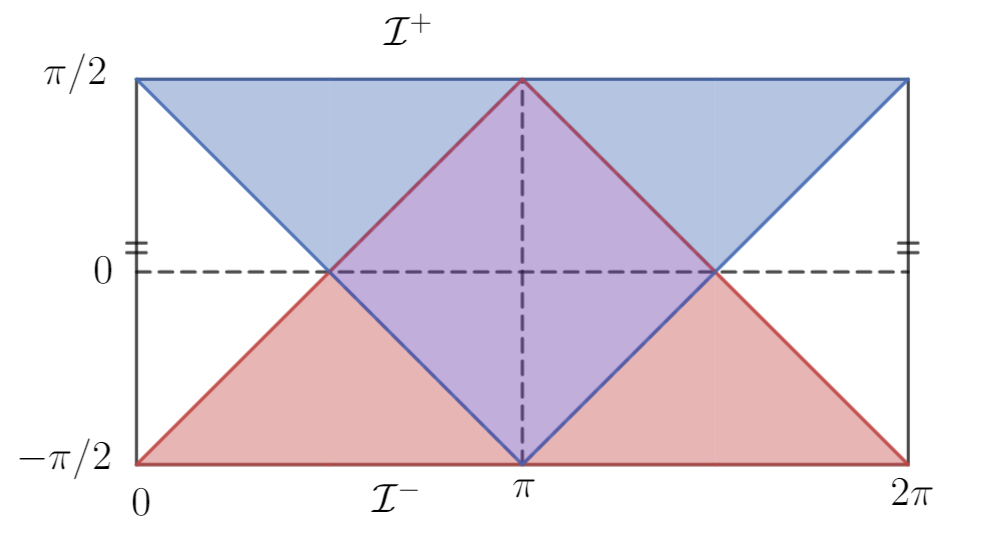
\includegraphics[width=12cm]{Penrose_dS2.PNG}
    \caption{Penrose diagram $dS_2$}
    \label{fig:penrose_dS2}
    
\end{figure}


Looking at the causal structure of the diagram, if we place an observer at $\phi=\pi$, then from $\tau=-\frac{\pi}{2}$ the blue area is the region that they can influence and at $\tau=\frac{\pi}{2}$ the red area is the region that can influence them. The purple area is the region which they can fully access which is called the static patch. The white area is the static patch for an observer at the other pole of the 1-sphere $\phi=0$, this area is completely causally disconnected from the observer at $\phi=\pi$.

\vspace{0.5cm}

\subsection{$dS_4$}


Now that we have reviewed $dS_2$ in detail we can look to the dimension we are interested in which is $dS_4$. We will follow a similar path to that of $dS_2$ by looking at the 4-sphere and then use a coordinate transformation to de Sitter geometry to give a more intuitive perspective of the isometries.


\subsubsection{de Sitter geometry $dS_4$}

To begin, we again take the example of the sphere, but instead of using the 2-sphere we will now use the 4-sphere with radius $l$, which has equation $x^ix_i=l^2$ where $i$ runs from 1 to 5. Taking the standard metric on $\rm I\!R^5$, $ds^2=dx^i dx_i$ and in the same way we did for the 2-sphere, we embed our coordinates onto the 4-sphere. Our embedding coordinates are as follows

\begin{equation}
\label{eq:embed 4-sphere1}    
    x_1= l \sin \phi_1 \hspace{2cm} \phi_1=\arctan \left( \frac{x_1}{\sqrt{x_2^2+x_3^2+x_4^2+x_5^2}} \right)
\end{equation}

\begin{equation}
\label{eq:embed 4-sphere2}    
    x_2= l \cos \phi_1 \sin \phi_2 \hspace{2cm} \phi_2=\arctan \left( \frac{x_2}{\sqrt{x_3^2+x_4^2+x_5^2}} \right)
\end{equation}

\begin{equation}
\label{eq:embed 4-sphere3}    
    x_3= l \cos \phi_1 \cos \phi_2 \sin \phi_3 \hspace{2cm} \phi_3=\arctan \left( \frac{x_3}{\sqrt{x_4^2+x_5^2}} \right)
\end{equation}

\begin{equation}
\label{eq:embed 4-sphere4}    
    x_4= l \cos \phi_1 \cos \phi_2 \cos \phi_3 \sin \phi_4 \hspace{2cm} \phi_4=\arctan \left( \frac{x_4}{x_5} \right)
\end{equation}

\begin{equation}
\label{eq:embed 4-sphere5}    
    \hspace{-5.5cm}
    x_5= l \cos \phi_1 \cos \phi_2 \cos \phi_3 \cos \phi_4 
\end{equation}

\vspace{0.5cm}

We can calculate the metric in these coordinates to find

\begin{equation}
\label{eq:4spheremetric}
    \frac{ds^2}{l^2}=d\phi_1^2+\cos^2 \phi_1 [d\phi_2^2+\cos^2 \phi_2(d\phi_3^2+\cos^2 \phi_3 d\phi_4^2)]
\end{equation}
\newline

Changing now to de Sitter geometry we simply change our embedding space to Minkowski spacetime ${\rm I\!R}^{1,2}$, with metric $ds^2= -dx_0^2 + dx_i^2$, and we change our embedding surface to a hyperboloid 


\begin{equation}
\label{eq:hyperboloid}
    -x_0^2 + \sum\limits_{i=1}^{4} x_i^2= l^2
\end{equation}

With the obvious choice of coordinate transformation $x_0\rightarrow it$, \eqref{eq:hyperboloid} becomes the equation for a sphere with radius $l$ and the Minkowski metric becomes the standard metric on $\rm I\!R^5$. Additionally with the coordinate transformation $\phi_1\rightarrow iT$ we get the metric

\begin{equation}
\label{eq:dS_4 metric1}
    \frac{ds^2}{l^2}=-dT^2+\cosh^2 T [d\phi_2^2+\cos^2\phi_2 (d\phi_3^2+\cos^2\phi_3 d\phi_4^2)]
\end{equation}

which can be simplified under trivial coordinate transformations to give

\begin{equation}
\label{eq:dS_4 metric}
    ds^2=-dT^2+l^2\cosh^2 \frac{T}{l} d\Omega^2_3
\end{equation}

where $d\Omega^2_3 \equiv d\psi^2+\sin^2\psi(d\theta^2+\sin^2\theta d\phi^2) $ is the round metric on the unit 3-sphere.


\subsubsection{Isometries of $dS_4$}

The manifest isometries for de Sitter space in this system are rotations and boosts, the translations that are Killing vectors of the Minkowski spacetime are lost in the embedding of the coordinates onto the hyperboloid, the Killing vectors can be represented in the form

\begin{equation}
\label{eq:dS_4 Killingrot}
    x_i\partial_j-x_j\partial_i
\end{equation}

\begin{equation}
\label{eq:dS_4 Killingboost}
    x_0\partial_i+x_i\partial_0
\end{equation}

\newpage

Working in 4 dimensions, $i$ and $j$ run from 1 to 4, the maximal number of  Killing vectors is $\frac{4(4+1)}{2}=10$ and since we have 4 boosts and 6 rotations the space is maximally symmetric, these are generators of the $SO(1,4)$ group.


We are able to change the coordinate system for these Killing vectors to the one we used in the metric \eqref{eq:dS_4 metric}, however this does not offer much more insight into the geometry of the de Sitter space. One of the important points to note is that as there are no translational Killing vectors, energy and momentum are not conserved and so the Hamiltonian is not well defined. In the next section we will see however, that there are metrics for de Sitter space where the manifest isometries include translations.

\subsubsection{Different metrics}

The metric \eqref{eq:dS_4 metric} is referred to as the global metric, and as we saw in section \textbf{2.1.6} we can compactify our coordinates to give us a different metric \eqref{compact_global_metric} which is called the conformal metric, in $dS_4$ this metric is 

\begin{equation}
\label{eq:conformal metric}
    ds^2=\frac{l^2}{\cos^2\tau}(-d\tau^2+d\Omega^2_3)
\end{equation}

\vspace{0.5cm}

The compactifiaction allows us to depict the Penrose diagram shown below.

\begin{figure}[h]
    \centering
    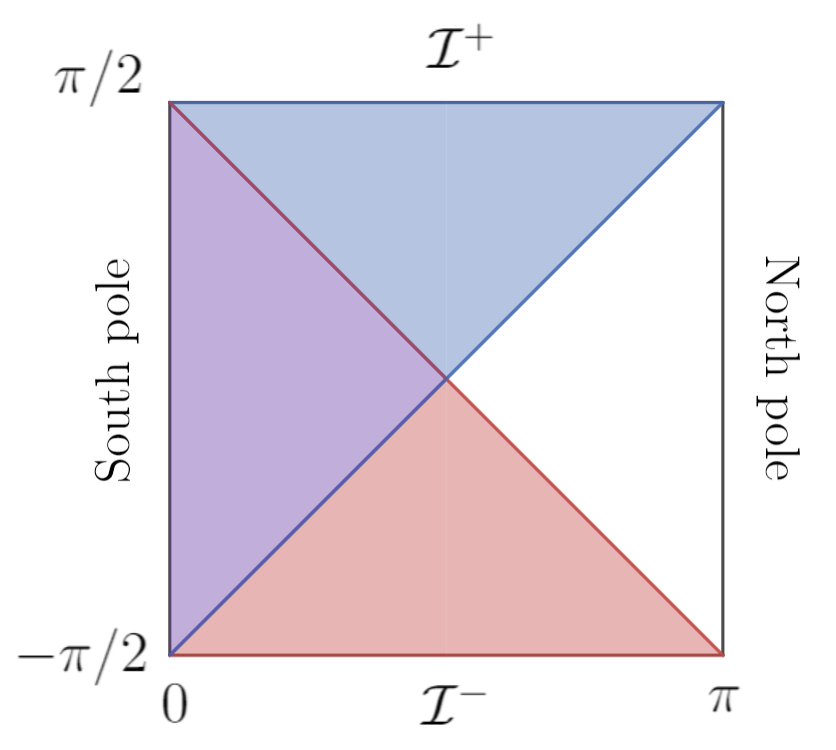
\includegraphics[width=8cm]{Penrose_dS4.PNG}
    \caption{Penrose diagram $dS_4$}
    \label{fig:penrose_dS4}
    
\end{figure}

For an observer at the south pole, the red area is the region that influences the observer and the blue area is the region which can be influenced by them. The purple area is the static path which is fully accessible to the observer and the white area is the region that is completely causally disconnected from them. Unlike the Penrose diagram for $dS_2$ this diagram is not topologically equivalent to a cylinder as the left and right sides of the diagram are not connected, but instead represent the poles of the 2-spheres, every interior point of the diagram is a 2-sphere, which contract from the infinite past to $\tau=0$, and expand from $\tau=0$ to the infinite future.



Another interesting metric to look at is the static metric, which holds a historic point of note. Around 1917 Einstein was looking for solutions to a static universe, as at the time there was no evidence for the universe expanding, he worked with de Sitter to find that introducing the cosmological constant gave a stable solution to a static universe. Later when it was discovered that the universe is not in fact static but expanding, he abandoned the cosmological constant, it was famously his ``biggest blunder'', however we now find relevance for it given the current observations showing the accelerated rate at which the universe is expanding. The metric is given by

\begin{equation}
\label{eq:static metric}
    ds^2=-\left(1-\frac{r^2}{l^2}\right)dt^2+\left(1-\frac{r^2}{l^2}\right)^{-1}dr^2+r^2d\Omega_2^2
\end{equation}


it only represents the static patch which is a quarter of the Penrose diagram from figure \ref{fig:penrose_dS4} shown by the purple area. We note that $\partial_t$ is a Killing vector in these coordinates, meaning the Hamiltonian is well defined so the energy is a conserved quantity. We also notice that this metric appears very similar to the Schwarzschild metric, and on the null surface $r=l$, represented as the diagonal red and blue lines in figure \ref{fig:penrose_dS4}, the norm of the Killing vector vanishes giving rise to a ``cosmological horizon''.
\newline

The final metric we will look at is the one we will use more in the later sections, as we will see the manifest isometries give important properties to the space. The metric is referred to as the planar metric, it covers half of the global geometry. We will be using the case where the metric covers the blue region from figure \ref{fig:penrose_dS4}, a light cone emanating from a point at $\mathcal{I}^-$, however we could equally take the red region, a light cone emanating from  a point at $\mathcal{I}^+$. To calculate the metric we can take the metric given by equation \ref{eq:conformal metric} and start by setting $\Tilde{\eta} = \tau -\frac{\pi}{2}$ which gives

\begin{equation}
\label{eta conformal}
    ds^2=\frac{l^2}{\cos^2(\Tilde{\eta}+\frac{\pi}{2})}(-d\Tilde{\eta}^2+d\Omega^2_3)
\end{equation}

Then since

$$\cos(x+\frac{\pi}{2})=-\sin(x)$$

\ref{eta conformal} becomes

\begin{equation}
\label{eta conformal2}
    ds^2=\frac{l^2}{\sin^2\Tilde{\eta}}(-d\Tilde{\eta}^2+d\Omega^2_3)
\end{equation}

we then introduce $\eta=\lambda\Tilde{\eta}$ where $\lambda \in {\rm I\!R}^+$ and take the limit as $\lambda \rightarrow \infty$

$$\lim_{\lambda\rightarrow\infty}\sin\frac{\eta}{\lambda}=\frac{\eta}{\lambda}$$

\newpage

which gives

\begin{equation}
\label{planar metric1}    
    ds^2=\frac{l^2 \lambda^2}{\eta^2}\left(-\frac{d\eta^2}{\lambda^2}+d\Omega^2_3 \right)
\end{equation}


we can then absorb the $\lambda^2$ term into the round metric, and we can chose a compact coordinate system for the round metric where the coordinates have both positive and negative values meaning when absorbing the $\lambda^2$ term, $\lambda^2d\Omega^2_3$ becomes $dx^2_i$, the standard metric on $\rm I\!R^3$ ($i=1,2,3$), giving the metric

\begin{equation}
\label{planar metric}
    ds^2=\frac{l^2}{\eta^2}(-d\eta^2+dx_i^2)
\end{equation}

Looking at the ranges for the coordinates we have already seen $x_i \in \rm I\!R^3$, for $\eta$ we find $-\frac{\pi}{2}<\tau<\frac{\pi}{2}$ gives $-\pi<\Tilde{\eta}<0$ meaning $\eta \in (-\infty,0)$. The manifest isometries of this metric are given in the A.2 appendix of \cite{Killing appendix}, we can intuitively see that spatial translations $\partial_i$ and rotations $\epsilon_{ijk}x^i\partial^j$ are isometries as the standard metric on $\rm I\!R^3$ features in the metric. Also if we take $\eta \rightarrow a\eta$ and $x \rightarrow ax$ where $a$ is a constant, the metric remains unchanged therefore dilations $-\eta\partial_{\eta}-x^i\partial_i$ are also an isometry. The final 3 isometries are called special conformal transformations, given by the Killing vectors $2x_i\eta\partial_{\eta}+[2x^jx_i+(\eta^2+\abs{\Vec{x}}^2)\delta^j_i]\partial_j$. We stated earlier that this metric will be used more in the later sections, this is because the isometries give a local property of $\rm I\!R^3$ which allows for Fourier analysis, which we will use to solve the Klein Gordon equation. 


\subsection{de Sitter action}

Starting by considering the action

\begin{equation}
\label{de Sitter action}
    S=\frac{1}{16\pi G} \int d^4x \sqrt{-g} (-R)
\end{equation}

we want to find the equations of motion, which we do by varying the action. Consider a matrix $A$, the determinant of the matrix can be written

\begin{equation}
\label{det A}   
    \det A=e^{\operatorname{tr}\ln A}
\end{equation}

which can be seen from diagonalizing $A$, it follows that

\begin{equation}
\label{ln det A}    
    \ln \det A= \operatorname{tr} \ln A
\end{equation}

\begin{equation}
 \label{delta det A}   
    \frac{\delta \det A}{\det A} = \operatorname{tr} \frac{\delta A}{A}
\end{equation}


then for $A=g_{\mu \nu}$, $\det A=g$ we get


\begin{equation}
\label{delta g}    
    \delta g=g g^{\mu \nu} \delta g_{\mu \nu}
\end{equation}

\newpage

which gives

\begin{equation}
\label{delta rt -g}    
    \delta \sqrt{-g}= -\frac{1}{2\sqrt{-g}}\delta g= -\frac{gg^{\mu \nu} \delta g_{\mu \nu}}{2\sqrt{-g}}=\frac{1}{2}\sqrt{-g} g^{\mu \nu} \delta g_{\mu \nu}=-\frac{1}{2}\sqrt{-g} g_{\mu \nu} \delta g^{\mu \nu}
\end{equation}


We also need to consider the $R=R_{\mu \nu} g^{\mu \nu}$ term

\begin{equation}
\label{delta R}
    \delta R= \delta g^{\mu \nu} R_{\mu \nu}+g^{\mu \nu} \delta R_{\mu \nu}
\end{equation}

therefore the variation of the action is

\begin{equation}
\label{variation of action}
    \delta S= - \frac{1}{16\pi G} \int d^4x \sqrt{-g} [(R_{\mu \nu} -\frac{1}{2} g_{\mu \nu} R)\delta g^{\mu \nu}+g^{\mu \nu}\delta R_{\mu \nu}]
\end{equation}



The $\delta R_{\mu \nu}$ term gives a total derivative, which when integrated only gives a boundary term that can be neglected giving the equations of motion


\begin{equation}
\label{Einstein tensor}
    R_{\mu \nu}-\frac{1}{2}g_{\mu \nu} R=0
\end{equation}

also known as the Einstein tensor $G_{\mu \nu}= R_{\mu \nu}-\frac{1}{2}g_{\mu \nu} R$. Now if we add a ``cosmological constant'' $\Lambda$ into the action given by \eqref{de Sitter action} as follows

\begin{equation}
\label{new action}
    S=\frac{1}{16\pi G} \int d^4x \sqrt{-g} (2\Lambda-R)
\end{equation}

it is clear to see the equations of motion become

\begin{equation}
\label{Einstein with lambda}
    R_{\mu \nu}-\frac{1}{2}g_{\mu \nu} R=-\Lambda g_{\mu \nu}
\end{equation}

This is the Einstein field equation in a vacuum, i.e. the stress energy tensor is zero $T_{\mu \nu}=0$. For Minkowski spacetime the cosmological constant is zero, but for de Sitter spacetime we require it to be positive $\Lambda>0$. The positive constant gives rise to an expanding universe at an accelerated rate as observed \cite{cosmoconst,cosmoval} the current approximation of the cosmological constant measured in our universe is $\Lambda \sim 10^{-122}$. We can check the metrics we have looked at in this section obey the equations of motion \eqref{Einstein with lambda} the calculations are given in Appendix A we find that $\Lambda=+3/l^2$ which is greater than zero as required.

\newpage

\section{Classical fields in de Sitter space}

We now move on to the field theory in a de Sitter background. Taking the Klein Gordon equation, we first need to alter it so that it is in the de Sitter background and then we look at solving the equation. We will look specifically at the early and late time limits of the solution and then observe what happens for specific masses.


\subsection{Klein Gordon equation}

The Klein Gordon equation is given by 

\begin{equation}
\label{Klein Gordon}    
    (\Box+m^2)\phi=0
\end{equation}

where $\Box$ is the d'Alembert operator. In flat space it becomes $\Box=-\partial^\mu\partial_\mu$, however as we are not in flat space we use covariant derivatives $\nabla_\mu$ instead. As $\phi$ is a scalar field the first derivative remains the same $\nabla_\mu\phi=\partial_\mu\phi$, but then as $\partial_\mu\phi$ is a vector quantity $\nabla^\mu\nabla_\mu\phi \neq \partial^\mu \partial_\mu\phi$. Instead we get

\begin{equation}
\label{covariant of vector}    
    \nabla^\mu\partial_\mu\phi=\partial^\mu \partial_\mu\phi+ \Gamma^\mu_{\mu\lambda} \partial^\lambda\phi
\end{equation}

$\Gamma$ is the Christoffel symbol given by

\begin{equation}
\label{Christoffel}
    \Gamma^k_{ij}=\frac{1}{2}g^{kl}(\partial_i g_{jl}+\partial_j g_{il}-\partial_l g_{ij})
\end{equation}

meaning 

\begin{equation}
\label{Christoffel1}    
    \Gamma^\mu_{\mu\lambda}=\frac{1}{2}g^{\mu\nu}(\partial_\lambda g_{\mu\nu}+\partial_\mu g_{\lambda\nu}-\partial_\nu g_{\mu\lambda})=\frac{1}{2} g^{\mu\nu}\partial_\lambda g_{\mu\nu}
\end{equation}

then using the formula

\begin{equation}
\label{formula}    
    \operatorname{Tr}(A^{-1}\partial_\lambda A)=\partial_\lambda \ln \det A
\end{equation}

where $A$ is an arbitrary matrix, we find 

\begin{equation}
\label{Christoffel2}    
    \Gamma^\mu_{\mu\lambda}=\frac{1}{2} \partial_\lambda \ln g = \frac{1}{\sqrt{g}}\partial_\lambda \sqrt{g}
\end{equation}

it follows that

\begin{equation}
\label{d'Al}
    \nabla^\mu\partial_\mu\phi=(\partial^\mu\partial_\mu+\frac{1}{\sqrt{g}}\partial_\lambda \sqrt{g}\partial^\lambda)\phi=\frac{1}{\sqrt{g}}\partial_\mu (g^{\mu\nu}\sqrt{g}\partial_\nu \phi)
\end{equation}

This can be seen in more detail on pages 106-107 in \cite{Weinberg}. This gives us the Klein Gordon equation in curved space as

\begin{equation}
\label{KG}
    \frac{1}{\sqrt{g}}\partial_\mu (g^{\mu\nu}\sqrt{g}\partial_\nu \phi)=m^2\phi
\end{equation}

\newpage

Taking the planar metric \eqref{planar metric} we find 

\begin{equation}
\label{gmunu}    
    g_{\mu\nu}=\frac{l^2}{\eta^2} \begin{pmatrix}
    -1&0&0&0\\
      0&1&0&0\\
      0&0&1&0\\
      0&0&0&1\\
    \end{pmatrix}
    \hspace{1cm}
    g^{\mu\nu}=\frac{\eta^2}{l^2} \begin{pmatrix}
    -1&0&0&0\\
      0&1&0&0\\
      0&0&1&0\\
      0&0&0&1\\
    \end{pmatrix}
\end{equation}

this also gives us 

\begin{equation}
\label{g}    
    g=-\frac{l^8}{\eta^8} \hspace{1cm} \sqrt{-g}=\frac{l^4}{\eta^4}
\end{equation}

(we need not concern ourselves with the minus sign in $\sqrt{-g}$) substituting \eqref{g} into \eqref{KG}  gives us

\begin{equation}
\label{DE1}
    \frac{\eta^4}{l^4}\partial_\eta(-\frac{l^2}{\eta^2}\partial_\eta\phi) +\frac{\eta^4}{l^4}\partial_{\Vec{x}} (\frac{l^2}{\eta^2}\partial_{\Vec{x}}\phi)=m^2\phi
\end{equation}

which simplifies to

\begin{equation}
\label{DE}    
    [-\eta^4\partial_\eta(\eta^{-2}\partial_\eta)+\eta^2\partial^2_{\Vec{x}}]\phi=m^2l^2\phi
\end{equation}

As stated earlier we can use a Fourier transformation to solve this differential equation, which we are able to do because of the local property of $\rm I\!R^3$ on the planar metric.
Note that the momentum $\Vec{k}$ that we are doing the Fourier decomposition with respect to is not the physical momentum, but is actually a coordinate momentum and the physical momentum is $\Vec{k}_{phys}=\eta\Vec{k}$.
Using the Fourier transform

\begin{equation}
\label{Fourier}    
    \phi(\eta,\Vec{x})=\int \frac{d^3k}{(2\pi)^3}e^{i\Vec{k}\cdot\Vec{x}}\phi(\eta,\Vec{k})
\end{equation}


 equation \eqref{DE} becomes

\begin{equation}
\label{DEFT}    
    [\eta^4\partial_\eta(\eta^{-2}\partial_\eta)+\eta^2k^2+m^2l^2]\phi(\eta,\Vec{k})=0
\end{equation}

where $k=\sqrt{\Vec{k}^2}$. The solution to this equation is given in Appendix B as

\begin{equation}
\label{phi1}    
    \phi_1(\eta,\Vec{k})=A(\Vec{k})\eta^{3/2}\mathcal{J}_\nu (\eta k)
\end{equation}

\begin{equation}
\label{phi2}
    \phi_2(\eta,\Vec{k})=B(\Vec{k})\eta^{3/2}\mathcal{Y}_\nu (\eta k)
\end{equation}

where $\nu^2=9/4-m^2l^2$, $A(\Vec{k})$ and $B(\Vec{k})$ are arbitrary functions, and $\mathcal{J}_\nu(x)$ and $\mathcal{Y}_\nu(x)$ are the Bessel functions of first and second kind respectively. We can combine our two solutions and substitute back into \eqref{Fourier} to give a general solution  

\begin{equation}
\label{genKGsol}    
    \phi(\eta,\Vec{x})= \int \frac{d^3k}{(2\pi)^3}\left[A(\Vec{k})\mathcal{J}_\nu (\eta k)+ B(\Vec{k})\mathcal{Y}_\nu (\eta k) \right]\eta^{3/2}e^{i \Vec{k}\cdot\Vec{x}}
\end{equation}

\newpage

The Bessel functions themselves are not simple to express, the most common way is a series expansion given by

\begin{equation}
\label{J(z)}    
    \mathcal{J}_\nu(z)=\left(\frac{z}{2}\right)^\nu \sum\limits_{k=0}^\infty (-1)^k \frac{(\frac{1}{4}z^2)^k}{k! \Gamma (\nu+k+1)}
\end{equation}

\vspace{0.5cm}

\begin{equation}
\label{Y(z)}    
    \mathcal{Y}_\nu(z)=\frac{\mathcal{J}_\nu(z)\cos(\nu\pi)-\mathcal{J}_{-\nu}(z)}{\sin(\nu\pi)}
\end{equation}

\vspace{0.5cm}

Because of the complexity in expressing these solutions we will find it more accessible to review specific areas of the solution, where it is expressed in a comprehensible manor. As such, in the next sections we proceed by reviewing the limiting behavior of the Bessel functions corresponding to the early and late time limits and then look to some specific values for $\nu$, which we notice assumes a complex value when $ml>3/2$, and as  we require $\phi(\eta,\Vec{x})$ to be real, the functions $A(\Vec{k})$ and $B(\Vec{k})$ will become complex too.

We note that when we come to quantizing the field later on, we will want  to have defined the conjugate momentum. So we now go about the calculation to find the conjugate momentum, we start by identifying the action for the Klein Gordon equation is 

\begin{equation}
\label{KGaction}    
    S=-\frac{1}{2}\int d^4x\sqrt{-g}(g^{\mu\nu}\partial_\mu\phi\partial_\nu\phi+m^2\phi^2) 
\end{equation}

from this we get the Lagrangian density

\begin{equation}
\label{Ldensity}    
    \mathcal{L}=-\frac{1}{2}\sqrt{-g}(g^{\mu\nu}\partial_\mu\phi\partial_\nu\phi+m^2\phi^2)=\frac{l^2}{2\eta^2} (\partial_\eta\phi)^2-\frac{l^2}{2\eta^2}(\partial_{\Vec{x}}\phi)^2-\frac{l^4}{2\eta^4}m^2\phi^2
\end{equation}

We note that this technically is not a true Lagrangian density as the $\Vec{x}$ coordinates are not the proper spatial lengths because $\eta$ weighs the proper length. With the following definition of the conjugate momentum 

$$\pi(\eta,\Vec{x})=\frac{\partial\mathcal{L}}{\partial(\partial_\eta\phi)}$$

we find 

\begin{equation}
\label{conjmom}    
    \pi(\eta,\Vec{x})=\frac{l^2}{\eta^2}\partial_\eta\phi
\end{equation}

using this we can also calculate the Hamiltonian density

\begin{equation}
\label{classicHam}    
    \mathcal{H}=\pi\partial_\eta\phi-\mathcal{L}=\frac{l^2}{2\eta^2} (\partial_\eta\phi)^2+\frac{l^2}{2\eta^2}(\partial_{\Vec{x}}\phi)^2+\frac{l^4}{2\eta^4}m^2\phi^2
\end{equation}

we see that it has an explicit time dependence and therefore the energy is not conserved which agrees with our earlier finding that the time translations $\partial_t$ are not Killing vectors of the global geometry.


\subsection{Solution to early time limit}

We look first at the early time limit where $\abs{\eta}\rightarrow\infty$, from \cite{limitingform} we see that 

\begin{equation}
\label{J(z) z>>1}    
    \mathcal{J}_\nu(z)\sim \sqrt{\frac{2}{\pi z}}\cos(z-\Phi)
\end{equation}

\begin{equation}
\label{Y(z) z>>1}    
    \mathcal{Y}_\nu(z)\sim \sqrt{\frac{2}{\pi z}}\sin(z-\Phi)
\end{equation}

where $\Phi=\frac{1}{2}\nu\pi+\frac{1}{4}\pi$ is a constant phase. We notice the behaviour is oscillatory for early times, but before substituting into our general solution we notice that a more appealing form can be seen when changing to the Hankel functions


\begin{equation}
\label{H1 z>>1}    
    \mathcal{J}_\nu(z)+i\mathcal{Y}_\nu(z)=H^{(1)}_\nu(z)\underrel[c]{z\to \infty}{\sim}\sqrt{\frac{2}{\pi z}}e^{i(z-\Phi)}
\end{equation}

\begin{equation}
\label{H2 z>>1}    
    \mathcal{J}_\nu(z)-i\mathcal{Y}_\nu(z)=H^{(2)}_\nu(z)\underrel[c]{z\to \infty}{\sim}\sqrt{\frac{2}{\pi z}}e^{-i(z-\Phi)}
\end{equation}

we can now substitute these approximations into our general solution to get the behaviour of early time limit as

\begin{equation}
\label{genKGsol1 eta>>1}    
    \phi(\eta,\Vec{x})=\int \frac{d^3k}{(2\pi)^3}\left[a(\Vec{k})\eta\sqrt{\frac{2}{\pi k}}e^{i(\eta k-\Phi+\Vec{k}\cdot\Vec{x})}+b(\Vec{k})\eta\sqrt{\frac{2}{\pi k}}e^{-i(\eta k-\Phi-\Vec{k}\cdot\Vec{x})} \right]
\end{equation}

where $a(\Vec{k})$ and $b(\Vec{k})$ are functions of $A(\Vec{k})$ and $B(\Vec{k})$, and as we require $\phi(\eta,\Vec{x})$ to be real $a^*(\Vec{k})=b(\Vec{-k})$ giving

\begin{equation}
\label{genKGsol eta>>1}    
    \phi(\eta,\Vec{x})=\int \frac{d^3k}{(2\pi)^3}\eta\sqrt{\frac{2}{\pi k}}\left[a(\Vec{k})e^{i(\eta k-\Phi+\Vec{k}\cdot\Vec{x})}+a^*(\Vec{k})e^{-i(\eta k-\Phi+\Vec{k}\cdot\Vec{x})} \right]
\end{equation}

This looks very similar to the solution to the Klein Gordon equation in flat space only multiplied by a factor of $\eta$ (although we note $\eta$ is not the proper time), meaning for the far past the scalar field has a similar solution to that of flat space.



\subsection{Solution to late time limit}

We can now look at the late time limit $\eta\rightarrow0$, from \cite{limitingform} we find

\begin{equation}
\label{J(z) z<<1}    
    \mathcal{J}_\nu(z)\sim \frac{(\frac{1}{2}z)^\nu}{\Gamma (\nu+1)}
\end{equation}

\begin{equation}
\label{Y(z) z<<1}    
    \mathcal{Y}_\nu(z)\sim -\frac{1}{\pi} \Gamma (\nu)(\frac{1}{2}z)^{-\nu}
\end{equation}

\newpage

substituting these approximations into our general solution to get the late time behaviour gives

\begin{equation}
\label{genKGsol eta<<1}    
    \phi(\eta,\Vec{x})=\int \frac{d^3k}{(2\pi)^3}\eta^{3/2}e^{i\Vec{k}\cdot\Vec{x}}\left(A(\Vec{k}) \frac{(\frac{1}{2}\eta k)^\nu}{\Gamma(\nu+1)}-B(\Vec{k})\frac{\Gamma(\nu)}{\pi(\frac{1}{2}\eta k)^\nu}\right)
\end{equation}

\vspace{1cm}

Another approach to solving the late time limit is to take the limit $\eta\rightarrow0$ of the differential equation \eqref{DE}. Following the solution from the lecture \cite{lecture1} we find when we take the limit $\eta\rightarrow0$ the $\eta^2\partial^2_{\Vec{x}}$ term is subleading, leaving us with an ordinary differential equation which is a lot easier to solve than the partial differential equation we have already worked through. We will now work through the solution to the following ODE

\begin{equation}
\label{ODE}    
    -\eta^4\partial_\eta(\eta^{-2}\partial_\eta)\phi(\eta,\Vec{x})=m^2l^2\phi(\eta,\Vec{x})
\end{equation}

we propose an ansatz for the solution to be of the form

\begin{equation}
\label{solODE}    
    \phi(\eta,\Vec{x})=\eta^\kappa a(\Vec{x})
\end{equation}

where $\kappa\in \mathbb{C}$ is a constant and as \eqref{ODE} is an ODE the solution can include an arbitrary function of $\Vec{x}$. Substituting \eqref{solODE} into \eqref{ODE} gives

\begin{equation}
\label{solsubODE}    
    -\kappa(\kappa-3)\eta^\kappa a(\Vec{x})=m^2l^2\eta^\kappa a(\Vec{x})
\end{equation}

giving the algebraic equation 

\begin{equation}
\label{algE}    
    \kappa^2-3\kappa+m^2l^2=0     
\end{equation}


which has solutions

\begin{equation}
\label{kappapm}    
    \kappa_{\Mypm}=\frac{3}{2}\Mypm\sqrt{\frac{9}{4}-m^2l^2}
\end{equation}

we can then substitute this into \eqref{solODE} to give the general solution

\begin{equation}
\label{gensolODE}    
    \phi(\eta,\Vec{x})=\eta^{\kappa_+}a_+(\Vec{x})+\eta^{\kappa_-}a_-(\Vec{x})+...
\end{equation}


The $+...$ at the end implies we have not got the complete solution, for example when $m^2l^2=\frac{9}{4}$, $\kappa$ is single valued, hence there would appear a $\log$ term to account for the degeneracy, however for our discussion we need not concern ourselves with the missing solutions. What we are interested in is how this solution behaves for different masses which will be covered in the following section.


\subsection{Solutions to different masses}

If we now take a closer look at specific masses for the solution to the late time limit equation \eqref{gensolODE}, we see that for particles with large masses  $ml>>\frac{3}{2}$, $\kappa$ is complex valued, intuitively we can regard heavy particles moving through the spacetime, as not sensing the curvature of the spacetime that much. It is the fact that $\kappa$ becomes complex for large masses that proves this intuition as it means that even in the late time limit the particle retains an oscillatory behaviour, bearing in mind that $\eta$ is not the proper time, when expressed in the terms of proper time $\eta=-e^{-T/l}$ where $T$ is the proper time. This oscillatory behaviour stops at the critical mass $m_cl=\frac{3}{2}$ where $\kappa_+=\kappa_-$, at this point instead of the oscillatory behaviour we are familiar with the solutions decay exponentially. The exponential decay of both modes is also the solution seen in the range $0<ml<\frac{3}{2}$. However for the case where the particle is massless, $\kappa_-=0$ meaning one of the modes is not decaying exponentially but leaves an imprint for arbitrarily late times, and it is this feature that allows us to have any chance of observing scale invariant fluctuations from the early cosmological era.




\newpage

\section{Quantum fields in de Sitter space}

Having gained an understanding of the classical scalar field, we move onto quantizing the field. Our procedure will follow that of canonical quantization,
however we notice that with the mode expansion of the classical field solution not being unique, we have a choice to make that affects how we define our vacuum state. We will use the mode expansion from equation \eqref{genKGsol eta>>1} meaning when $a(\Vec{k})$ acts on the vacuum state, it is annihilated.


\subsection{Quantization}


To quantize our field we promote $\phi(\eta,\Vec{x})$ and $\pi(\eta,\Vec{x})$ to operators obeying the commutation relations

\begin{equation}
\label{cc1}
    [\phi(\eta,\Vec{x}),\phi(\eta,\Vec{y})]=0
\end{equation}

\begin{equation}
\label{cc2}
    [\pi(\eta,\Vec{x}),\pi(\eta,\Vec{y})]=0
\end{equation}

\begin{equation}
\label{cc3}
    [\phi(\eta,\Vec{x}),\pi(\eta,\Vec{y})]=i\delta^{(3)}(\Vec{x}-\Vec{y})
\end{equation}

the coefficients $a(\Vec{k})$ and $a^*(\Vec{k})$ are also promoted to operators and obey the commutation relations 

\begin{equation}
\label{cc4}    
    [a(\Vec{k}),a(\Vec{k}')]=0
\end{equation}

\begin{equation}
\label{cc5}    
    [a^\dagger(\Vec{k}),a^\dagger(\Vec{k}')]=0
\end{equation}


\begin{equation}
\label{cc6}    
    [a(\Vec{k}),a^\dagger(\Vec{k}')]=(2\pi)^3\delta^{(3)}(\Vec{k}-\Vec{k'})
\end{equation}


and we have that $a(\Vec{k})\ket{0}=0$, which allows us to generate the Fock space in the same way we would in flat space. Now using equation \eqref{genKGsol} and following a similar procedure that lead to the equation \eqref{genKGsol eta>>1} we get 

\begin{equation}
\label{quantphi}    
    \phi(\eta,\Vec{x})=\int \frac{d^3k}{(2\pi^3)}\eta^{3/2}[a(\Vec{k})e^{i\Vec{k}\cdot\Vec{x}}H_\nu^{(1)}(\eta k)+a^\dagger(\Vec{k})e^{-i\Vec{k}\cdot\Vec{x}}H_\nu^{(2)}(\eta k)]
\end{equation}

we can separate this into the creation and annihilation parts which we will use in the calculation of the two point function

\begin{equation}
\label{quantphi-}    
    \phi^-(\eta,\Vec{x})=\int \frac{d^3k}{(2\pi^3)}\eta^{3/2}a(\Vec{k})e^{i\Vec{k}\cdot\Vec{x}}H_\nu^{(1)}(\eta k)
\end{equation}

\begin{equation}
\label{quantphi+}    
    \phi^+(\eta,\Vec{x})=\int \frac{d^3k}{(2\pi^3)}\eta^{3/2}a^\dagger(\Vec{k})e^{-i\Vec{k}\cdot\Vec{x}}H_\nu^{(2)}(\eta k)
\end{equation}

\newpage

\subsection{Two point function}

We finally get to calculating the two point function

\begin{equation}
\label{2pnt}    
    \bra{0}\phi(\eta,\Vec{x})\phi(\eta',\Vec{y})\ket{0}
\end{equation}

by definition 

\begin{equation}
\label{normalorder and com}    
    \phi(\eta,\Vec{x})\phi(\eta',\Vec{y})=:\phi(\eta,\Vec{x})\phi(\eta',\Vec{y}):+[\phi^-(\eta,\Vec{x}),\phi^+(\eta',\Vec{y})]
\end{equation}

the colons represent normal ordering, where the annihilation operators are moved to the right, meaning when this is substituted into \eqref{2pnt} it gives us

\begin{equation}
\label{2point}    
    \bra{0}[\phi^-(\eta,\Vec{x}),\phi^+(\eta',\Vec{y})]\ket{0}
\end{equation}

\begin{equation}
\label{2pointcalc}
    =\eta^{3/2}\eta'^{3/2}\int \frac{d^3k}{(2\pi)^3}\frac{d^3k'}{(2\pi)^3}H^{(1)}_\nu(\eta k)H^{(2)}_\nu(\eta'k')e^{i(\Vec{k}\cdot\Vec{x}-\Vec{k'}\cdot\Vec{y})}\bra{0}[a(\Vec{k}),a^\dagger(\Vec{k'})]\ket{0}
\end{equation}

substituting in the relation \eqref{cc6} and integrating over the $k'$ coordinate gives us

\begin{equation}
\label{2pointsol}    
    \bra{0} \phi(\eta,\Vec{x})\phi(\eta',\Vec{y})\ket{0}=(\eta\eta')^{3/2}\int \frac{d^3k}{(2\pi)^3}H^{(1)}_\nu(\eta k)H^{(2)}_\nu(\eta'k)e^{i\Vec{k}\cdot(\Vec{x}-\Vec{y})}
\end{equation}

As this is not an easy integral to solve, we can again look at the approximation of the solution in the early and late time limits. Before we change to the limiting behaviour we can look at changing to spherical polar coordinates to perform the integration, in doing so we use $\Vec{a}\cdot\Vec{b}=\abs{a}\abs{b}\cos \theta$, where $\Vec{a}$ and $\Vec{b}$ are vectors and $\theta$ is the angle between them, we get

\begin{equation}
\label{2pointsolsp}    
    \bra{0} \phi(\eta,\Vec{x})\phi(\eta',\Vec{y})\ket{0}=\frac{(\eta\eta')^{3/2}}{(2\pi)^3}\int^\infty_0 dr\int_0^{2\pi} d\phi \int_0^\pi d\theta r^2 \sin \theta H^{(1)}_\nu(\eta r)H^{(2)}_\nu(\eta'r)e^{i r \abs{\Vec{x}-\Vec{y}}\cos\theta}
\end{equation}

then doing the integral over $d\phi$ gives a factor of $2\pi$, we use Mathematica to calculate the integral over $d\theta$ which leaves us with

\begin{equation}
\label{2pointsolr}    
    \bra{0} \phi(\eta,\Vec{x})\phi(\eta',\Vec{y})\ket{0}=\frac{2}{\abs{\Vec{x}-\Vec{y}}}\frac{(\eta\eta')^{3/2}}{(2\pi)^2}\int^\infty_0 dr r \sin(r \abs{\Vec{x}-\Vec{y}}) H^{(1)}_\nu(\eta r)H^{(2)}_\nu(\eta'r)
\end{equation}

It is at this point that the integral becomes too complicated to solve without taking the early and late time limits, we will start by considering the early time limit where the Hankel functions are approximated by equations \eqref{H1 z>>1} and \eqref{H2 z>>1} which gives 
\begin{equation}
\label{2pointsol eta>>1}    
    \bra{0} \phi(\eta,\Vec{x})\phi(\eta',\Vec{y})\ket{0}=\frac{8}{\abs{\Vec{x}-\Vec{y}}}\frac{(\eta\eta')}{(2\pi)^3}\int^\infty_0 dr  \sin(r \abs{\Vec{x}-\Vec{y}}) e^{ir(\eta-\eta')} 
\end{equation}

\newpage

Again we can use Mathematica to solve this integral to give us the final solution for the two point function in the early time limit as

\begin{equation}
\label{2pointfullsol eta>>1}    
    \bra{0} \phi(\eta,\Vec{x})\phi(\eta',\Vec{y})\ket{0}=\frac{8}{\abs{\Vec{x}-\Vec{y}}}\frac{(\eta\eta')}{(2\pi)^3} \frac{\abs{\Vec{x}-\Vec{y}}}{\abs{\Vec{x}-\Vec{y}}^2-(\eta-\eta')^2}=\frac{1}{\pi^3} \frac{\eta\eta'}{\abs{\Vec{x}-\Vec{y}}^2-(\eta-\eta')^2}
\end{equation}

Now we can look at specific cases of $x-y$, we see for a timelike interval $\Vec{x}-\Vec{y}=0$ and $\eta-\eta'=t$, we get 

\begin{equation}
\label{2point eta>>1 x-y=0}    
    \bra{0} \phi(\eta,\Vec{x})\phi(\eta',\Vec{y})\ket{0}=-\frac{1}{\pi^3} \frac{\eta\eta'}{t^2}
\end{equation}


comparing this to the solution in flat space given the limit $t\rightarrow\infty$ has the approximate solution $e^{-imt}$. We can also look at the spacelike interval $\Vec{x}-\Vec{y}=r$ and $\eta-\eta'=0$, we get 


\begin{equation}
\label{2point eta>>1 eta-eta'=0}    
    \bra{0} \phi(\eta,\Vec{x})\phi(\eta',\Vec{y})\ket{0}=\frac{1}{\pi^3} \frac{\eta\eta'}{\abs{\Vec{x}-\Vec{y}}^2}
\end{equation}

we compare this to our solution in flat space given the limit $r\rightarrow\infty$ which has the approximate solution $e^{-mr}$.
\newline
We now move onto the late time limit, we first need to find the limiting behaviour of the Hankel functions are. We take the limits of the Bessel functions from equations \eqref{J(z) z<<1} and \eqref{Y(z) z<<1} and change to the form of the Hankel functions using the relations seen in \eqref{H1 z>>1} and \eqref{H2 z>>1} which gives

\begin{equation}
\label{H1 z<<1}    
    H^{(1)}_\nu(z)\sim \frac{(\frac{1}{2}z)^\nu}{\Gamma(\nu+1)}-\frac{i}{\pi}\frac{\Gamma(\nu)}{(\frac{1}{2}z)^\nu}
\end{equation}

\begin{equation}
\label{H2 z<<1}    
    H^{(2)}_\nu(z)\sim \frac{(\frac{1}{2}z)^\nu}{\Gamma(\nu+1)}+\frac{i}{\pi}\frac{\Gamma(\nu)}{(\frac{1}{2}z)^\nu}
\end{equation}

From equation \eqref{2pointsolr} we want to calculate $H^{(1)}_\nu(\eta r)H^{(2)}_\nu(\eta'r)$ which gives 

\begin{equation}
\label{H1H2}    
    \frac{(\frac{1}{2}k)^{2\nu}(\eta\eta')^\nu}{\Gamma^2(\nu+1)}+\frac{i}{\pi\nu}(\frac{\eta}{\eta'})^\nu-\frac{i}{\pi\nu}(\frac{\eta'}{\eta})^\nu+\frac{1}{\pi^2}\frac{\Gamma^2(\nu)}{(\frac{1}{2}k)^{2\nu}(\eta\eta')^\nu}
\end{equation}

however in the limit $\eta\rightarrow0$ the first three terms are subleading so can be disregarded, giving us

\begin{equation}
\label{2pointsolr eta<<1}    
    \bra{0} \phi(\eta,\Vec{x})\phi(\eta',\Vec{y})\ket{0}=\frac{2}{\abs{\Vec{x}-\Vec{y}}}\frac{(\eta\eta')^{3/2}}{(2\pi)^2}\int^\infty_0 dr r \sin(r \abs{\Vec{x}-\Vec{y}}) \frac{1}{\pi^2}\frac{\Gamma^2(\nu)}{(\frac{1}{2}r)^{2\nu}(\eta\eta')^\nu}
\end{equation}

simplifying to give

\begin{equation}
\label{2pointsol eta<<1}    
    \bra{0} \phi(\eta,\Vec{x})\phi(\eta',\Vec{y})\ket{0}=\frac{2^{(2+2\nu)}}{\abs{\Vec{x}-\Vec{y}}}\frac{(\eta\eta')^{3/2-\nu}}{(2\pi)^3}\frac{\Gamma^2(\nu)}{\pi}\int^\infty_0 dr r^{1-2\nu} \sin(r \abs{\Vec{x}-\Vec{y}}) 
\end{equation}


\newpage

Using Mathematica to solve this integral gives 

\begin{equation}
\label{2pointfinalsol eta<<1}    
    \bra{0} \phi(\eta,\Vec{x})\phi(\eta',\Vec{y})\ket{0}=\frac{2^{(2+2\nu)}}{\abs{\Vec{x}-\Vec{y}}}\frac{(\eta\eta')^{3/2-\nu}}{(2\pi)^3}\frac{\Gamma^2(\nu)}{\pi} \abs{\Vec{x}-\Vec{y}}^{2\nu-2}\Gamma(2-2\nu) \sin(\pi\nu)
\end{equation}

\begin{equation}
\label{2pointfinalsol2 eta<<1}    
    =\frac{2^{(2+2\nu)}}{\pi}\frac{\sin(\pi\nu)}{(2\pi)^3}\Gamma^2(\nu) \Gamma(2-2\nu)\abs{\Vec{x}-\Vec{y}}^{2\nu-3} (\eta\eta')^{3/2-\nu}
\end{equation}

\begin{equation}
\label{2pointfinalsol3 eta<<1}    
    =f(\nu)\abs{\Vec{x}-\Vec{y}}^{2\nu-3} (\eta\eta')^{3/2-\nu}
\end{equation}


where $f(\nu)$ is the function o $\nu$ that cleans up the look of the solution, this solution is conditional though and is only valid for $\frac{1}{2}<\Re(\nu)<\frac{3}{2}$. We can again look at our solution in the timelike interval $\Vec{x}-\Vec{y}=0$ and $\eta-\eta'=t$, we get 


\begin{equation}
\label{2point eta<<1 x-y=0}
    \bra{0} \phi(\eta,\Vec{x})\phi(\eta',\Vec{y})\ket{0}=f(\nu) (\eta\eta')^{3/2-\nu}
\end{equation}


we can also note that for the massless particle $\nu=\frac{3}{2}$, although the function $f(\nu)$ is not analytic at this point, we notice that the solution has no explicit time dependence or spatial separation dependence, meaning the correlations do not dilute with time, which gives cosmologists a chance of observing the fluctuations from the inflationary era.  

\newpage

\section{Conclusion}

In a brief summary of the paper we see we have reviewed the geometry of the de Sitter background,looking in detail at the isometries of the spacetime. We find that as a result of $\partial_t$ not being a Killing vector of the global geometry the energy is not a conserved quantity, which is then enforced with our later finding that the Hamiltonian is explicitly time dependent. When solving the classical Klein Gordon equation we find that even in the late time limit for significantly massive particles $ml>\frac{3}{2}$ the solution still gives oscillatory behaviour. We finally finish by quantizing our field and comparing our solution with those of flat space, we find an important point that for a massless particle the correlation does not dilute with time and therefore offers the opportunity for observations from the inflationary era of our universe. Further work that was not explored in this paper could include looking at an interacting theory such as the three point function.


\section*{Acknowledgements}

I thank my supervisor Dr Dionysios Anninos for his help and support throughout my work on this project. I also thank my tutor Prof. Sameer Murthy for his guidance throughout this academic year. And a general thank you to the theoretical physics group that are part of the Mathematics department at King's College London, for the teaching they have given me that has allowed me to acquire the necessary knowledge required to undertake this project.


\newpage

\section*{Appendix A}

The following appendix is a 3 page pdf file from the program ``Wolfram Mathematica 11.3" using the package ``GRQUICK". It confirms that all of the metrics from the section 2.2.3 ``Different metrics" obey the equations of motion given by equation \eqref{Einstein with lambda} from section 2.3 ``de Sitter action". We have used the ansatz that $\Lambda=+3/l^2$ which is given in \cite{de Sitter musings}. The function ``Einstein$[i,j]$" gives the $[i,j]$th component of the left hand side of equation \eqref{Einstein tensor} i.e. the Einstein tensor. The ``Metric$[i,j]$" function gives the $[i,j]$th component of the metric tensor.

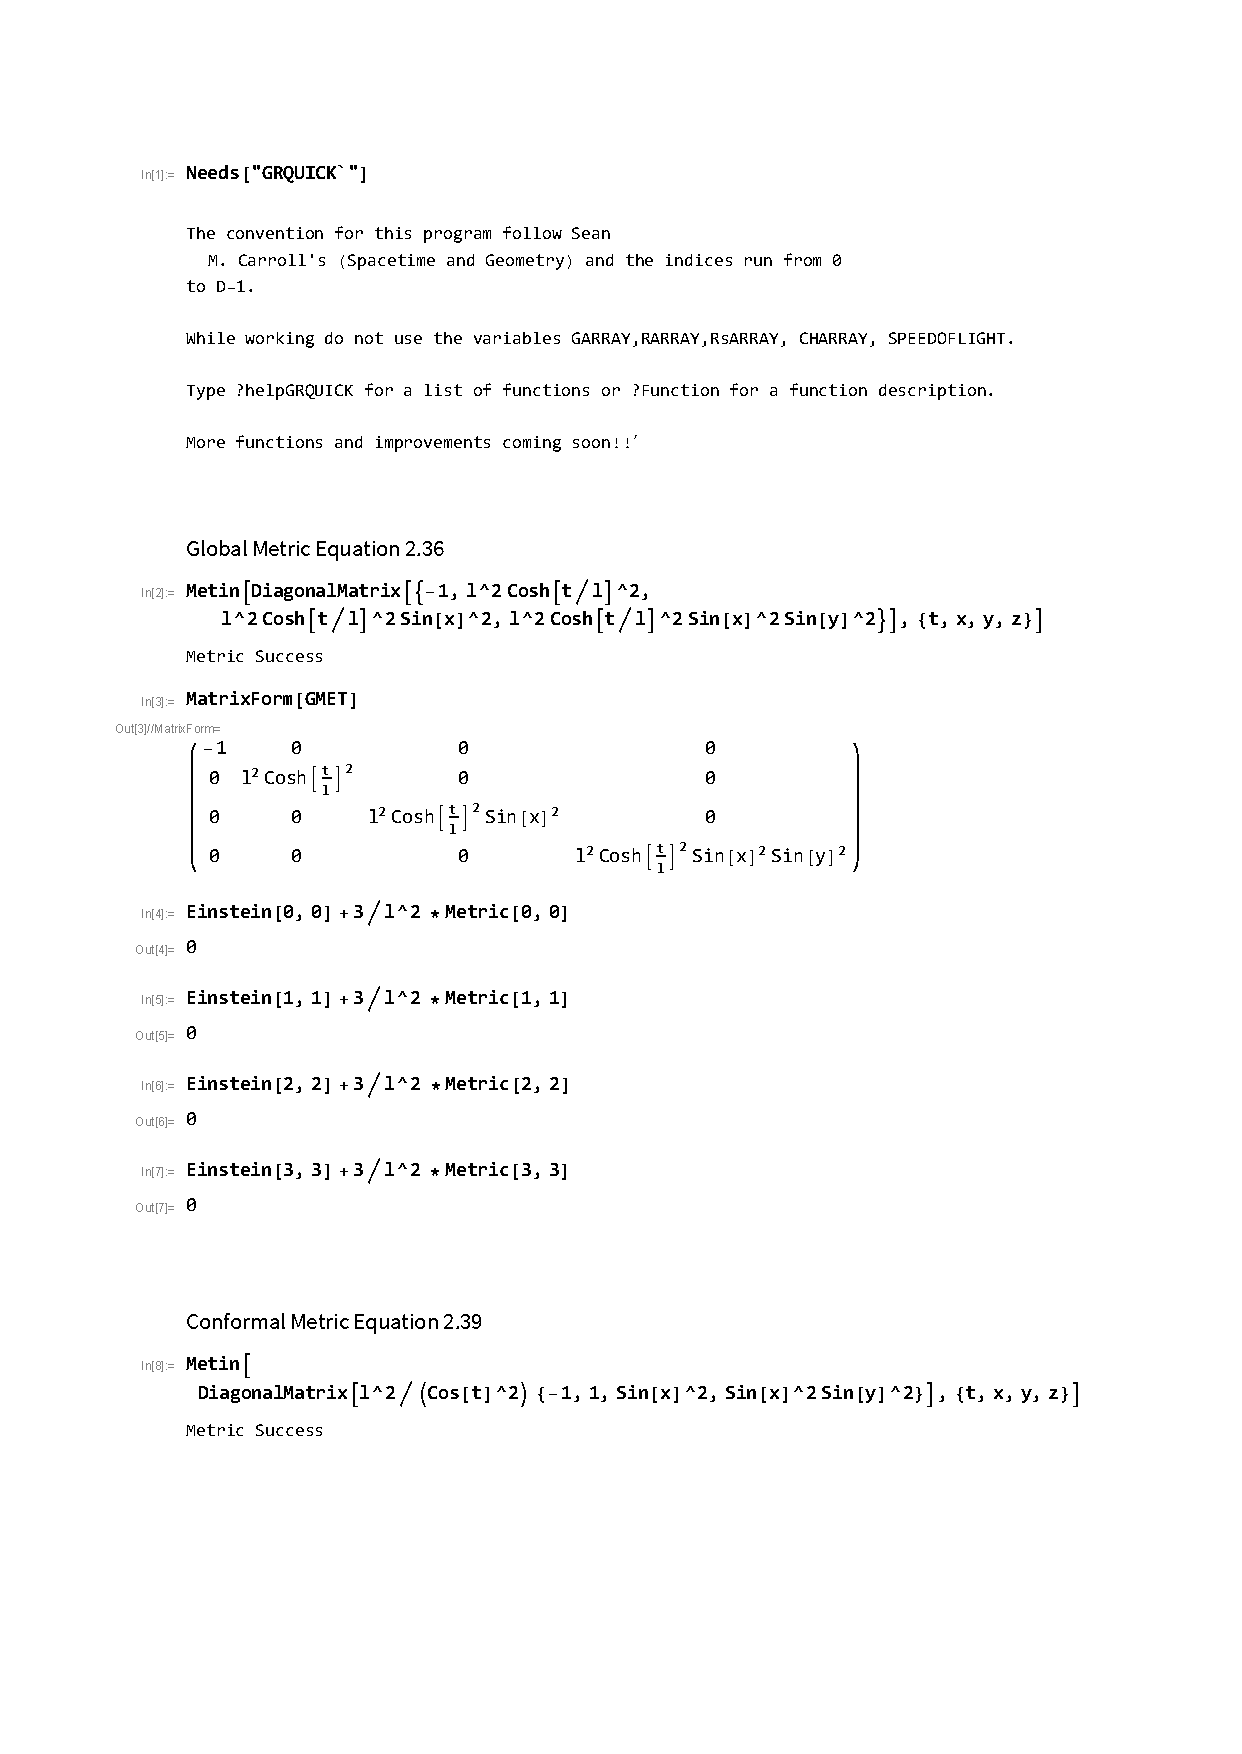
\includepdf[pages=-]{Metric EoM}

\newpage

\section*{Appendix B}

This appendix follows the solution to the differential equation \eqref{DEFT}. We first expand the equation to give

$$[\eta^2\partial_\eta^2-2\eta\partial_\eta+\eta^2k^2+m^2l^2]\phi(\eta,\Vec{k})=0$$

we identify that the solutions to this are going to be Bessel functions, as such we look for transformations that get the equation into the form

$$[x^2\partial_x^2+x\partial_x+(x^2-\alpha^2)]y(x)=0$$

we make a transformation to the field $\phi=\eta^{3/2}\Tilde{\phi}$ which gives 

$$[\eta^2\partial_\eta^2-2\eta\partial_\eta+\eta^2k^2+m^2l^2]\eta^{3/2}\Tilde{\phi}(\eta,\Vec{k})=0$$

which is solved to give

$$\eta^{7/2}\partial_\eta^2\Tilde{\phi}(\eta,\Vec{k})+\eta^{5/2}\partial_\eta\Tilde{\phi}(\eta,\Vec{k})-\frac{9}{4}\eta^{3/2}\Tilde{\phi}(\eta,\Vec{k})+(\eta^2k^2+m^2l^2)\eta^{3/2}\Tilde{\phi}(\eta,\Vec{k})=0$$

if we now divide through by $\eta^{3/2}$ we get

$$[\eta^2\partial_\eta^2+\eta\partial_\eta+(-\frac{9}{4}+\eta^2k^2+m^2l^2)]\Tilde{\phi}(\eta,\Vec{k})=0$$

now if we make the change of coordinates $\Tilde{\eta}=\eta k$ we find 

$$\partial_\eta=\partial_{\Tilde{\eta}}\frac{d\Tilde{\eta}}{d\eta}=k\partial_{\Tilde{\eta}}$$

which gives

$$[{\Tilde{\eta}}^2\partial_{\Tilde{\eta}}^2+{\Tilde{\eta}}\partial_{\Tilde{\eta}}+(\Tilde{\eta}^2+m^2l^2-\frac{9}{4})]\Tilde{\phi}(\Tilde{\eta},\Vec{k})=0$$

which is of the form of the Bessel equation so if we set $\nu^2=\frac{9}{4}-m^2l^2$, our solutions are

$$\Tilde{\phi}_1(\Tilde{\eta},\Vec{k})=A(\Vec{k})\mathcal{J}_\nu (\Tilde{\eta})$$

$$\Tilde{\phi}_2(\Tilde{\eta},\Vec{k})=B(\Vec{k})\mathcal{Y}_\nu (\Tilde{\eta})$$

which when we convert back to our original form gives us the solutions to equation \eqref{DEFT} as

$$\phi_1(\eta,\Vec{k})=A(\Vec{k})\eta^{3/2}\mathcal{J}_\nu (\eta k)$$

$$\phi_2(\eta,\Vec{k})=B(\Vec{k})\eta^{3/2}\mathcal{Y}_\nu (\eta k)$$



\newpage

\begin{thebibliography}{}

    \bibitem{supernova1}
    S. Perlmutter et al. [Supernova Cosmology Project Collaboration], “Measurements of Omega
    and Lambda from 42 high redshift supernovae,” Astrophys. J. 517, 565 (1999) [astroph/9812133].


    \bibitem{supernova2}
    A. G. Riess et al. [Supernova Search Team Collaboration], “Observational evidence from supernovae for an accelerating universe and a cosmological constant,” Astron. J. 116, 1009 (1998)
    [astro-ph/9805201].

    \bibitem{cosmoconst}
    R. Bousso, “TASI Lectures on the Cosmological Constant,” Gen. Rel. Grav. 40, 607 (2008)
    [arXiv:0708.4231 [hep-th]].

    
    \bibitem{future structure}
    K. Nagamine and A. Loeb, “Future Evolution of Nearby Large-Scale Structure in a Universe
    Dominated by a Cosmological Constant,” arXiv:astro-ph/0204249v3 12 Nov 2002
    
    \bibitem{inflation1}
    D. Baumann, “TASI Lectures on Inflation,” arXiv:0907.5424 [hep-th].
    
    \bibitem{inflation2}
    S. Tsujikawa, “Introductory Review of Cosmic Inflation,” arXiv:hep-ph/0304257
    
    \bibitem{Killing appendix}
    G. Sengor and C. Skordis, “Unitarity at the Late time Boundary of de Sitter,” arXiv:1912.09885 [hep-th]
    
    \bibitem{cosmoval}
    J. D. Barrow and D. J. Shaw, “The Value of the Cosmological Constant,” arXiv:1105.3105 [gr-qc]
    
    \bibitem{Weinberg}
    S. Weinberg, “Gravitation and Cosmology principles and applications of the general theory of relativity,” (1972)

    
    \bibitem{limitingform}
    Dlmf.nist.gov. 2020. DLMF: 10.7 Limiting Forms. [online] Available at: https://dlmf.nist.gov/10.7 [Accessed 9 September 2020].
    
    \bibitem{lecture1}
    Dionysios Anninos- Aspect of De Sitter Space (Lecture)- 
    International Centre for Theoretical Sciences Bengaluru, India- (2018)
    
    \bibitem{de Sitter musings}
    D. Anninos, “De sitter musings,” 	arXiv:1205.3855 [hep-th] May 2012.
    
    \bibitem{lts}
    D. Anninos, T. Anous, D. Z. Freedman, G. Konstantinidis, “Late-time Structure of the Bunch-Davies De Sitter Wavefunction,” arXiv:1406.5490 [hep-th]
    
    \bibitem{hsds}
    D. Anninos, F. Denef, R. Monten, Z. Sun, “Higher Spin de Sitter Hilbert Space,” arXiv:1711.10037 [hep-th]
    
    \bibitem{kv}
    Mu-Lin Yan, “Killing Vectors in Spacetime of the De Sitter Invariant Special Relativity,” arXiv:1707.04153 [gr-qc]
    
    \bibitem{irr}
    D. Anninos, D. M. Hofman, “Infrared Realization of dS2 in AdS2,” 	arXiv:1703.04622 [hep-th]
    
    \bibitem{ltsbd}
    G. Konstantinidis, R. Mahajan, E. Shaghoulian, “Late-time Structure of the Bunch-Davies FRW Wavefunction,” arXiv:1608.06163 [hep-th]
    
    \bibitem{cgds}
    Y. Kim, C. Y. Oh, N. Park, “Classical Geometry of De Sitter Spacetime : An Introductory Review,” 	arXiv:hep-th/0212326
    
    \bibitem{fskg}
    K. Yagdjian, A. Galstian, “Fundamental Solutions for the Klein-Gordon Equation in de Sitter Spacetime,” 	arXiv:0803.3074 [math.AP]
    
    \bibitem{dssh}
    Hep.physics.uoc.gr. 2020. [online] Available at: http://hep.physics.uoc.gr/mideast3/
    talks/alishahiha.pdf?fbclid=IwAR3BnAvIgKZXnYLYuSaH3jYSn39t5kD0gEH8Iu-YmwOHAstwvejWXw8oqwk [Accessed 9 September 2020].
    
    \bibitem{lecture2}
    Dionysios Anninos- Topics in de Sitter space (Lecture)-CERN Winter School- (2018)
    
\end{thebibliography}




\end{large}
\end{document}
